% Created 2021-08-11 mer. 22:29
% Intended LaTeX compiler: pdflatex
\documentclass{beamer}
\usepackage[utf8]{inputenc}
\usepackage[T1]{fontenc}
\usepackage[french]{babel}
\usepackage{mlkkone}
\usepackage{lmodern}
\usepackage{multicol}
\usepackage{hyperref}
\usepackage{MnSymbol,wasysym}
\usepackage{verbatim}
\usepackage{caption}

\mode<presentation>{
  \usetheme{Montpellier}
  \setbeamercovered{transparent}
  \setbeamertemplate{section in toc}[sections numbered]
  \setbeamertemplate{subsection in toc}[square]
}

\useoutertheme{infolines} 

\makeatother
\setbeamertemplate{footline}
{
  \leavevmode% 
  \hbox{%
    \begin{beamercolorbox}[wd=.333\paperwidth,ht=2.25ex,dp=1ex,center]{author in head/foot}%
      \usebeamerfont{author in head/foot} \insertshortauthor \hspace{1em} (\insertshortinstitute)
    \end{beamercolorbox}%
    \begin{beamercolorbox}[wd=.466\paperwidth,ht=2.25ex,dp=1ex,center]{title in head/foot}%
      \usebeamerfont{title in head/foot}\insertshorttitle
    \end{beamercolorbox}
    \begin{beamercolorbox}[wd=.2\paperwidth,ht=2.25ex,dp=1ex,center]{date in head/foot}%
      \usebeamerfont{date in head/foot}\insertshortdate\hspace*{3em}
      \insertframenumber{} / \inserttotalframenumber\hspace*{1ex}
    \end{beamercolorbox}}%
  \vskip0pt%
}
\makeatletter
\usetheme{Montpellier}
\author{Malik Koné}
\date[]{mercredi 28 juillet 2021}
\title{Blockchain}
\subtitle{Bitcoin et Crypto-monnaies, au-delà du buzz}
\hypersetup{
  pdfauthor={Malik Koné},
  pdftitle={Blockchain},
  pdfkeywords={},
  pdfsubject={},
  pdfcreator={Emacs 27.2 (Org mode 9.4.6)}, 
  pdflang={French}}
\begin{document}


{
  \usebackgroundtemplate{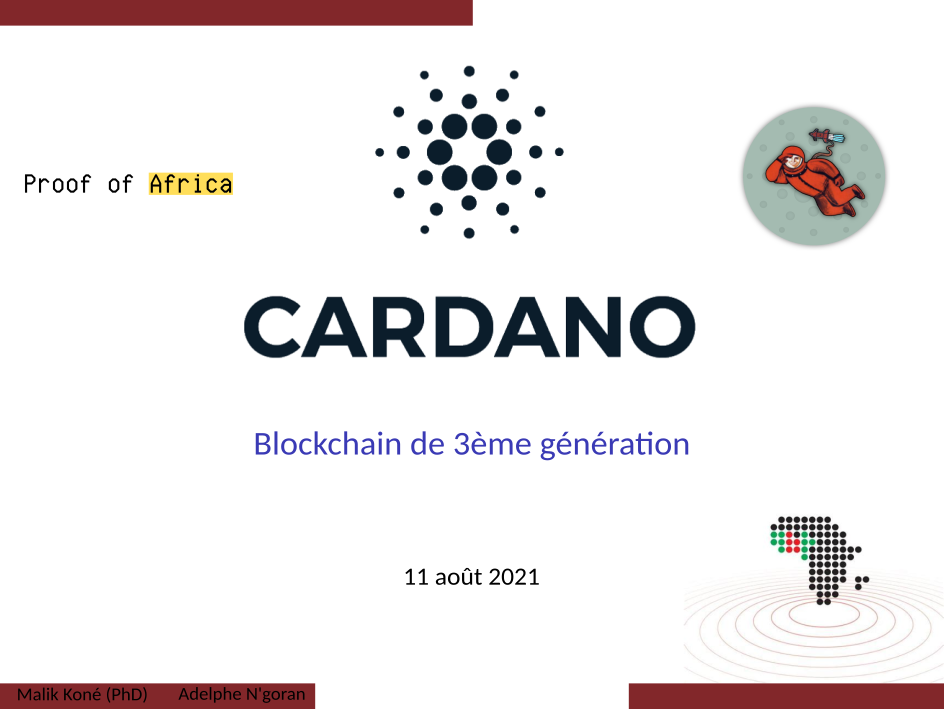
\includegraphics[height=\paperheight]{./page_de_garde_uvci}}
  \frame[plain]{
  }
}

\begin{frame}{Plan}
  \tableofcontents
\end{frame}


\section{Introduction}
\label{sec:org32a77db}
\begin{frame}[label={sec:org49a1e98}]{Les concepts de base}
  \begin{center}
    \includegraphics[width=\textwidth]{Images/cryptographics/anatomy-of-a-chain-1.png}
  \end{center}

  \begin{columns}
    \begin{column}{0.48\columnwidth}
      \begin{block}{Blockchain}
        \begin{itemize}
        \item <1>Enregistrements décentralisés
        \item <1>Algorithmes de consensus
        \item <1>Cryptographie
        \item <1>Applications distribuées (dApp)
        \end{itemize}
      \end{block}
    \end{column}
    \begin{column}{0.48\columnwidth}
      \begin{block}{Token-économie}
        \begin{itemize}
        \item <2> Tokens ou jetons
        \item <2> Marchés financiers
        \item <2-> Portefeuilles éléctroniques (\href{https://yoroi-wallet.com}{Yoroi-wallet})
        \end{itemize}
      \end{block}
    \end{column}
  \end{columns}
\end{frame}

\section{Bitcoin : Blockchain de 1\iere{} génération}
\label{sec:org863a5c7}
\begin{frame}[label={sec:org5d99e7b}]{La blockchain du Bitcoin}
  \begin{verse}
    Toute action engendre une réaction (3\ieme{} loi de Newton)\\
  \end{verse}
\end{frame}
\begin{frame}[label={sec:org3969a5e}]{La Naissance du Bitcoin}
  \begin{columns}
    \begin{column}{0.70\columnwidth}
      \begin{block}{From: Satoshi Nakamoto satoshi@vistomail.com}
        \begin{verbatiminput}
          SSubject: Bitcoin P2P e-cashe paper\\
          Newsgroups: gmane.comp.encryption.general\\
          Date: Friday 31st October 2008 18:10:00 UTC\\
          ~\\
          I've been working on a new electronic cash system that's fully peer-to-peer, with no trusted third party.
        \end{verbatiminput}
      \end{block}
    \end{column}
    \begin{column}{0.30\columnwidth}
      \begin{block}{Cyber-Anarchisme}
        \begin{center}
          \includegraphics[width=.7\linewidth]{Images/assange.jpg}
        \end{center}
      \end{block}
    \end{column}
  \end{columns}
\end{frame}

\begin{frame}[label={sec:orgc45170e}]{Quel problème résoud la 1\iere{} blockchain ?}
  \begin{block}{Connecter, échanger, librement}
    \only<1>{
      \begin{center}
        \includegraphics[width=.7\textwidth]{./Images/layers.png}
      \end{center} 
    }

    \only<2>{
      \begin{center}
        \includegraphics[width=.7\textwidth]{./Images/layers_ssl.png}
      \end{center}
    }

    \only<3>{
      \begin{center}
        \includegraphics[width=.7\textwidth]{./Images/layers_btc.png}
      \end{center} 
    }
  \end{block}
\end{frame}


\begin{frame}[label={sec:org91227f5}]{Les obstacles}
  \only<1->{
    \begin{block}{La double dépense}
    }
    \only<1>{
      \begin{center}
        \includegraphics[width=.8\linewidth]{Images/double_depense.png}
      \end{center}
    }
    \only<2->{
    \end{block}
    \begin{block}{L'attaque de Sybil}
      \begin{center}
        \includegraphics[width=\linewidth]{Images/sybillschema.png}
      \end{center}
    }
  \end{block}
\end{frame}


\begin{frame}[label={sec:org960f420}]{Comment le problème est résolu ?}
  \begin{center}
    \includegraphics[width=\textwidth]{Images/cryptographics/anatomy-of-a-chain-1.png}
  \end{center}

  \begin{block}{avec une blokchain}
    \only<1>{
      Un journal comptable d'enregistrements,
      \begin{itemize}
      \item organisés en blocks infalsifiables
      \item qui s'enchainent les uns aux autres,
      \item de façon unique,
      \item dans un réseau publique et décentralisé.
      \end{itemize}
    }
    \only<2->{
    \end{block}
    \begin{block}{et des rôles (Chaum 92)}
      \begin{itemize}
      \item Utilisateurs
      \end{itemize}

      \begin{itemize}
      \item Acteurs (mineur)
      \end{itemize}

      \begin{itemize}
      \item Décideurs
      \end{itemize}

      \begin{itemize}
      \item Empereurs  (\href{https://github.com/bitcoin/bitcoin}{MIT bitcoin-core developpeurs} et d'autres\ldots{})
      \end{itemize}

    }
  \end{block}
\end{frame}

\begin{frame}[label={sec:org58ca4f0}]{Comment le problème est-il résolu ?}
  \begin{block}{\href{https://www.blockchain.com/btc/block/0}{Block 0}}
    \begin{center}
      \includegraphics[width=.7 \textwidth]{Images/btc_block0.png}
    \end{center}
    \begin{block}{Le \href{https://www.blockchain.com/btc/block/123456}{block 123 456}}
    \end{block}
  \end{block}
\end{frame}

\begin{frame}[label={sec:org17d81ce}]{Pour faire une transaction}
  \begin{figure}[ht]
    \centering
    \includegraphics<1>[width=.6\textwidth]{Images/cryptographics/tx}
    \includegraphics<2>[width=.6\textwidth]{Images/cryptographics/block}
    \includegraphics<3>[width=\textwidth]{Images/cryptographics/Anatomy-of-a-block2}    
    \includegraphics<4>[width=\textwidth]{Images/cryptographics/anatomy-of-a-chain-1}
  \end{figure}

  \only<1>{
    Tx:  ".00012300 BTC pour Binta, signé Amadou"
  }
  \only<2>{
    Les mineurs inclu la tx dans un bloc et cherchent un \alert{bon} \emph{nonce}
  }
  \only<3>{
    Le 1\ier{} mineur à trouver un \alert{bon} \emph{nonce}, publie le bloc
    \begin{itemize}
    \item il contient une récompense (\emph{coinbase})
    \end{itemize}
  }
  \only<4>{
    Les autres mineurs:
    \begin{itemize}
    \item Vérifie le nonce
    \item ajoutent le nouveau block à la chaine
    \item recommencent la course pour valider un nouveau bloc de transactions et obtenir une récompense
    \end{itemize}
  }
\end{frame}
\begin{frame}[label={sec:orgcba4c84}]{La pizza à 10 000 BTC}
  \begin{center}
    \includegraphics[width=.7\linewidth]{Images/pizza_1millions.jpg}
  \end{center}
  \begin{itemize}
  \item le 18 mai 2010, \href{https://bitcointalk.org/index.php?topic=137.msg1195}{laslo sur bitcointalk.org}
  \item Le Bitcoin est devenu une l'unité de compte d'\href{https://www.blockchain.com/btc/address/1XPTgDRhN8RFnzniWCddobD9iKZatrvH4}{journal comptable ouvert} infalsifiable
  \end{itemize}
  \begin{block}{A quand son garba payé en QR code?}
  \end{block}
\end{frame}
\begin{frame}[label={sec:org48b1e57}]{Limites de la blockchain bitcoin 1/5}
  \begin{block}{Coût énergétique}
    \begin{center}
      \includegraphics[width=\textwidth]{Images/mining-farm-bitcoin.jpg}
    \end{center}
  \end{block}
\end{frame}

\begin{frame}[label={sec:org0c58574}]{Limites de la blockchain bitcoin 2/5}
  \begin{block}{Concentration du \href{https://www.blockchain.com/charts/pools}{hashrate} (juin 2021)}
    \begin{center}
      \includegraphics[width=.6\textwidth]{Images/hashrate_juin21.png}
    \end{center}
  \end{block}
\end{frame}

\begin{frame}[label={sec:org5d6af00}]{Limites de la blockchain Bitcoin 3/5}
  \begin{block}{Politique: forks}
    \begin{center}
      \includegraphics[width=\textwidth]{Images/cryptographics/blockchain-hard-fork.png}
    \end{center}
  \end{block}
\end{frame}

\begin{frame}[label={sec:orgdcb07cf}]{Limites de la Blockchain bitcoin 4/5}
  \begin{block}{Vitesse de traitement des transactions}
    \begin{center}
      \includegraphics[width=\textwidth]{Images/cryptographics/the-scaling-issue.png}
    \end{center}
  \end{block}
\end{frame}

\begin{frame}[label={sec:org88e1887}]{Limites de la Blockchain bitcoin 5/5}
  \begin{block}{Jeux d'instructions limités}
    \begin{center}
      \includegraphics[width=.9\textwidth]{Images/automate_simple.jpeg}
    \end{center}
  \end{block}
\end{frame}

\section{Etherum : Blockchain de 2\ieme{} génération}
\label{sec:orgcaf736a}
\begin{frame}[label={sec:orgda9df99}]{Blockchain de 2\ieme{} génération : Etherum}
  \begin{verse}
    Un système d'exploitation décentralisé\\
  \end{verse}
\end{frame}
\begin{frame}[label={sec:orgcd4bf8f}]{Distributed applications (smart contracts)}
  \begin{columns}
    \begin{column}{0.60\columnwidth}
      \begin{block}{DEFI}
        \only<1>{
          \begin{itemize}
          \item Services financiers décentralisés (DeFI)
          \item Financement participatif
          \item Dépots de garantis (emprunt)
          \item Création de marchés de pairs à pairs
          \item Paiement internationaux
          \end{itemize}
        }
        \only<2>{
          \begin{itemize}
          \item Logistique
          \item Identité numérique
          \item Monnaie dirigée
          \item Objets connectés
          \end{itemize}
        }
      \end{block}
    \end{column}
    \begin{column}{0.39\columnwidth}
      \begin{block}{}
        \only<1>{
          \begin{center}
            \includegraphics[width=.9\textwidth]{Images/defi_service.jpeg}
          \end{center}
        }
        \only<2>{
          \begin{center}
            \includegraphics[width=.9\textwidth]{Images/defi_coins.jpeg}
          \end{center}
        }
      \end{block}
    \end{column}
  \end{columns}
\end{frame}

\begin{frame}[label={sec:org9b18c95}]{Blockchain de 2\ieme{} génération : Etherum}
  \only<1>{
    \begin{center}
      \includegraphics[width=.8\linewidth]{Images/turing_schema.png}
    \end{center}
  }

  \only<2>{
    \begin{center}
      \includegraphics[width=.6\linewidth]{Images/solidity.png}
    \end{center}
  }

  \only<3>{
    \begin{center}
      \includegraphics[width=.6\linewidth]{Images/logos/ethereum_classic_logo.jpg}
    \end{center}
  }
  \begin{block}{}
    \begin{itemize}
    \item <1-> Machine Turing complet
    \item <2-> dApps et smart-contracts (solidity)
    \item <3> ETH, ETC et gaz
    \end{itemize}
  \end{block}
\end{frame}

\begin{frame}[label={sec:orgc5f9255}]{Les limites d'Etherum}
  \begin{columns}
    \begin{column}{0.39\columnwidth}
      \begin{block}{}
        \begin{itemize}
        \item Pas assez sécurisé
        \item Coûteux
        \item Difficile à améliorer
        \end{itemize}
      \end{block}
    \end{column}
    \begin{column}{0.60\columnwidth}
      \begin{block}{}
        \begin{center}
          \includegraphics[width=.9\linewidth]{Images/dao.png}
        \end{center}
      \end{block}
    \end{column}
  \end{columns}
\end{frame}



\section{Cardano : blockchain de 3\ieme{} génération}
\label{sec:org61221b4}
\begin{frame}[label={sec:org918e93a}]{Cardano: blockchain de 3\ieme{} génération}
  \begin{verse}
    1, 2, et \(\cdots{}\) 3 !\\
  \end{verse}
\end{frame}
\begin{frame}[label={sec:orgc83cd94}]{Originalité du projet}
  \begin{block}{1\ier{} blockchain scientifique}
    \begin{center}
      \includegraphics[width=.5\linewidth]{Images/logos/cardano_logo.png}
    \end{center}

    \begin{center}
      \includegraphics[width=\linewidth]{Images/cardano/roadmap_small.png}
    \end{center}
  \end{block}
\end{frame}


\begin{frame}[label={sec:orgaa015b3}]{Les fondations}
  \begin{center}
    \includegraphics[width=\linewidth]{Images/cardano/roadmap_step1.png}
  \end{center}

  \begin{block}{Ouroboros POS}
    \centering
    \includegraphics[width=.4\textwidth]{Images/logos/ouroboros}
  \end{block}
\end{frame}

\begin{frame}[label={sec:orgc310498}]{La décentralisation}
  \begin{center}
    \includegraphics[width=\linewidth]{Images/cardano/roadmap_step2.png}
  \end{center}

  \begin{block}{Stacking et pools}
    \centering
    \includegraphics[width=.6\textwidth]{Images/cardano/green_pool.jpeg}
  \end{block}
\end{frame}

\begin{frame}[label={sec:org0c2e3e9}]{Les smart-contract}
  \begin{center}
    \includegraphics[width=\linewidth]{Images/cardano/roadmap_step3.png}
  \end{center}

  \centering
  \includegraphics[width=.6\textwidth]{Images/plutus_haskell.png}
\end{frame}

\begin{frame}[label={sec:org78f4fe6}]{La mise à l'échelle}
  \begin{center}
    \includegraphics[width=\linewidth]{Images/cardano/roadmap_step4.png}
  \end{center}

  \centering
  \includegraphics[width=.5\textwidth]{Images/cardano/daedalus_ada_cardano_w}
\end{frame}

\begin{frame}[label={sec:orga2ff3d7}]{La gouvernance}
  \begin{center}
    \includegraphics[width=\linewidth]{Images/cardano/roadmap_step5.png}
  \end{center}

  \begin{block}{Vote et Trésor}
    \centering
    \includegraphics[width=.6\textwidth]{Images/cardano/catalyst.jpeg}
  \end{block}
\end{frame}





\section{Token-economie}
\label{sec:org2cc307c}
\begin{frame}[label={sec:orged54339}]{}
  \begin{verse}
    Un révolution techno-sociale ?\\
  \end{verse}
\end{frame}
\begin{frame}[label={sec:orga4b9574}]{La monnaie}
  \begin{columns}
    \begin{column}{0.44\columnwidth}
      \begin{block}{}
        \begin{block}{Qu'est ce que la monnaie ?}
          \only<1-2>{
            \begin{itemize}
            \item <1>unité de valeur, de change et de compte
            \item <2>un jeu d'écriture
            \end{itemize}
          }
        \end{block}

        \begin{block}{Une histoire de confiance (Aglietta \& Orléan 1998)}
          \only<3-4>{
            \begin{itemize}
            \item <3>L'obligation (autorité)
            \item <3>La confiance (éthique)
            \item <4>L'habitude (méthodique)
            \end{itemize}
          }
        \end{block}
      \end{block}
    \end{column}
    \begin{column}{0.55\columnwidth}
      \begin{block}{}
        \only<1>{
          \begin{center}
            \includegraphics[width=.9\textwidth]{Images/yap_Stone_Money.jpg}
          \end{center}
        }
        \only<2>{
          \begin{center}
            \includegraphics[width=.9\textwidth]{Images/continental_note.png}
          \end{center}
        }
        \only<3>{
          \begin{center}
            \includegraphics[width=.9\textwidth]{Images/bceao_meyliet_kone.jpg}
          \end{center}
        }
        \only<4>{
          \begin{center}
            \includegraphics[width=.9\textwidth]{Images/piece.jpg}
          \end{center}
        }
      \end{block}
    \end{column}
  \end{columns}
\end{frame}
\begin{frame}[label={sec:orgf65db3b}]{Les Crypto-monnaies}
  \begin{center}
    \includegraphics[width=.9\linewidth]{Images/logos/cryptos.jpeg}
  \end{center}

  \begin{columns}
    \begin{column}{0.43\columnwidth}
      \begin{block}{Jetons (tokens)}
        \begin{itemize}
        \item <1> de protocole
        \item <2> utilitaires ou applicatifs
          \begin{itemize}
          \item \emph{stable coins}
          \item non \emph{fongible} (NFT)
          \end{itemize}
        \end{itemize}
      \end{block}
    \end{column}

    \begin{column}{0.55\columnwidth}
      \begin{block}{Marchés des crypto-monnaies}
        \begin{itemize}
        \item <3> le marché du crédit: \$~250~billions
        \item <3> Le marché des actions: \$~80~billions
        \item <3> le marché de l'or: \$~7~billions
        \item <3> \alert{le marché des cryptos: \$~1~500~milliards}
        \end{itemize}
      \end{block}
    \end{column}
  \end{columns}
\end{frame}


\begin{frame}[label={sec:orgc72683b}]{Comment avoir des ADA ?}
  \begin{columns}
    \begin{column}{0.45\columnwidth}
      \begin{block}{avec des BTC}
        \begin{itemize}
        \item Acheter des BTC
        \item Plateformes d'échange pair à pair ex. \href{https://localbitcoins.com/fr/}{localbitcoins}
        \item Maisons de change (\href{https://ayael-entreprise.com/}{ayael} au plateau)
        \end{itemize}
      \end{block}
    \end{column}

    \begin{column}{0.55\columnwidth}
      \begin{block}{Directement}
        \begin{itemize}
        \item Un vendeur, un donnateur physique (ex. moi)
        \item Acheter en ligne sur des plateformes reconnues
          \begin{itemize}
          \item \href{https://www.binance.com/fr}{binance} (CH), \href{https://www.kraken.com/}{kraken} (A), \href{https://www.coinbase.com/fr/}{coinbase} (USA)
          \item voir \href{https://www.coingecko.com/fr}{coingecko} pour classement
          \item avec CB d'une autre zone monétaire que FCFA
          \end{itemize}
        \end{itemize}
      \end{block}
    \end{column}
  \end{columns}
\end{frame}

\begin{frame}[label={sec:org4c2743f}]{Comment garder ses ADA  ?}
  \begin{columns}
    \begin{column}{0.55\columnwidth}
      \begin{block}{}
        \begin{block}{\href{https://daedaluswallet.io}{Daedalus} (noeud complet)}
          \begin{center}
            \includegraphics[width=.2\linewidth]{Images/cardano/daedalus.png}
          \end{center}

          \only<2>{
          \end{block}
          \begin{block}{Ouvrir un porte-feuille éléctronique}
            \begin{enumerate}
            \item Installer yoroi-wallet pour android ou plugin de navigateur
            \item Noter les mots de sauvegarde
            \item Partager votre adresse publique
            \item Recevez des ADA ou lovelace
            \end{enumerate}
          }
        \end{block}
      \end{block}
    \end{column}
    \begin{column}{0.43\columnwidth}
      \begin{block}{\href{https://yoroi-wallet.com}{Yoroi} (portefeuille léger)}
        \begin{center}
          \includegraphics[width=.7\linewidth]{Images/cardano/o-yoroi.jpg}
        \end{center}
      \end{block}
    \end{column}
  \end{columns}
\end{frame}

\begin{frame}[label={sec:org085f67a}]{Délégation et stacking}
  \begin{description}
  \item[{Gagner +5 à 7\% d'ADA en minant}] 

  \item[{Déléguez}] à \alert{une pool} c'est se regrouper pour valider ensemble des transactions, contre rémunération
  \end{description}
  \begin{block}{}
    \begin{columns}
      \begin{column}{0.48\columnwidth}
        \begin{block}{\href{https://www.abobolaispool.com/}{Abobolais Pool}}
          \begin{center}
            \includegraphics[width=.4\linewidth]{Images/logos/abobolais_pool.png}
          \end{center}
        \end{block}
      \end{column}

      \begin{column}{0.48\columnwidth}
        \begin{block}{\href{https://cardano.afrikpool.org/}{Afrikpool}}
          \begin{center}
            \includegraphics[width=.2\linewidth]{Images/logos/afrikpool.png}
          \end{center}
        \end{block}
      \end{column}
    \end{columns}
  \end{block}
  \begin{block}{}
    \begin{columns}
      \begin{column}{0.48\columnwidth}
        \begin{block}{\href{https://adapools.org/pool/683e89fa1bcde139504b11fbfd914f8ebe9b8db2678b3da0abdcb2f1}{POA}}
          \begin{center}
            \includegraphics[width=.4\linewidth]{Images/cardano/proof_of_africa.png}
          \end{center}
        \end{block}
      \end{column}

      \begin{column}{0.48\columnwidth}
        \begin{block}{\href{https://adapools.org/pool/b62ecc8ce7e46c4443b63b91fffaeb19f869d191a7d2381087aaa768}{STKH1}}
          \begin{center}
            \includegraphics[width=.2\linewidth]{Images/cardano/to_moon_stkh.png}
          \end{center}
        \end{block}
      \end{column}
    \end{columns}
  \end{block}
\end{frame}

\section{Conclusion}
\label{sec:orgbd8c608}
\begin{frame}[label={sec:orgccfd267}]{Conclusion}
  \begin{block}{Cardano}
    \begin{itemize}
    \item \href{https://roadmap.cardano.org/en/}{Plan de déploiement Cardano}
    \item \href{https://explorer.cardano.org/}{Explorateur de bloc pour Cardano}
    \item \href{//github.com/input-output-hk/cardano-node}{Cardano-node (github)}
    \end{itemize}
    \begin{block}{Délégation}
      \begin{itemize}
      \item \url{https://adapools.org}
      \item formulaire :\url{https://forms.gle/vjaGwDx3oQLrToLo6}
      \end{itemize}
    \end{block}
  \end{block}

  \begin{block}{Evènements Blockchains}
    \begin{itemize}
    \item mars 2022 \href{https://blockchainafrica.co/blockchain-africa-conference-johannesburg-2/}{Conférence Blockchain en Afrique du Sud}
    \end{itemize}
  \end{block}
\end{frame}

\begin{frame}[label={sec:org0d82882}]{C'est l'heure de l'air drop}
  \begin{enumerate}
  \item Créer un wallet (suivre les instructions)
  \item Copier l'adresse publique dans le formulaire ci-dessou
  \item \url{https://tinyurl.com/anzy45fk}
  \item Transférer à un ami
  \item Déléguer ensemble
  \end{enumerate}

  \begin{columns}
    \begin{column}{0.40\columnwidth}
      \begin{block}{Yoroi-wallet}
        \begin{center}
          \includegraphics[width=.9\textwidth]{Images/logo-yoroi-wallet.jpg}
        \end{center}
      \end{block}
    \end{column}
    \begin{column}{0.4\columnwidth}
      \begin{block}{Merci à tous}
        \begin{center}
          \includegraphics[width=.9\textwidth]{Images/cardano/daedalus_ada_cardano_w.png}
        \end{center}
      \end{block}
    \end{column}
  \end{columns}
\end{frame}
\end{document}